\chapter{Detector and Physics at Future Linear Colliders}
\label{chap:Detector}

\chapterquote{ILC will be built next year}%
{Mysterious person}%: Blackwood's Magazine May 1830





Since the discovery of a particle consistent with being the SM Higgs boson in LHC at 2012 \cite{Aad:2012tfa,Chatrchyan:2012ufa}, our understanding of Standard Model has improved greatly. Yet limited by the underlying QCD interaction from proton-anti-proton collision, one has great difficulty to measure the properties of the Higgs precisely. Next generation electron-positron linear collider could hopefully make precision measurements of the Higgs sector and the Top quark sector \cite{Abramowicz:2013tzc}.

The leading candidates for next generation electron-positron linear collider are the International Linear Collider (ILC) \cite{Brau:2007zza}, and the Compact Linear Collider (CLIC) \cite{Linssen:2012hp}. The ILC has developed two detector models, namely the International Large Detector (ILD) \cite{Abe:2010aa} and the Silicon Detector (SiD) \cite{Aihara:2010zz}. The CLIC has developed two slightly modified detector models based on ILD and SiD \cite{Linssen:2012hp}. One key common feature of these next generation electron-positron linear colliders is the high granular calorimeter, which provides a great spatial resolution at the cost of the energy resolution. Particle flow algorithms (PFA) benefit from the spatial resolution from calorimeters, together with tracking information, to provide excellent a jet energy resolution. PandoraPFA, the most complicated and the best performing one, provides a jet energy resolution of less than 3.5\%, which is required for W/Z separation \cite{Thomson:2009rp,Marshall:2013bda}.


overall

Future linear collider

ILC

CLIC



\section{Physics at ILC}

Tau - LC relavence tau

Double higgs


general higgs field

Lagrangian

current constraint

single higgs coupling measurement done in higgs

Double higgs measurement

The main mechanism for double Higgs production %in \epem collisions
%at high energy CLIC ($\sqrt{s}>$\SI{1}{\TeV}) is via $WW$-fusion ($\epem\to HH\nu\overline{\nu}$). The main Feynman diagrams contributing to the process are illustrated in Figure . %The cross section for the process increases with the centre-of-mass energy: from \SI{0.15}{\fb} at $\sqrt{s}=$\SI{1.4}{\TeV} to \SI{0.59}{\fb} at $\sqrt{s}=$\SI{3}{\TeV}, assuming a %Higgs mass of \SI{126}{GeV}.




\section{Physics at CILC}

current constraint

single higgs coupling measurement done in higgs

Double higgs measurement

The main mechanism for double Higgs production %in \epem collisions
%at high energy CLIC ($\sqrt{s}>$\SI{1}{\TeV}) is via $WW$-fusion ($\epem\to HH\nu\overline{\nu}$). The main Feynman diagrams contributing to the process are illustrated in Figure . %The cross section for the process increases with the centre-of-mass energy: from \SI{0.15}{\fb} at $\sqrt{s}=$\SI{1.4}{\TeV} to \SI{0.59}{\fb} at $\sqrt{s}=$\SI{3}{\TeV}, assuming a %Higgs mass of \SI{126}{GeV}.




\section{ILD vs SID}



\section{CLIC vs ILC}

Due to the similarities of the two two linear collider programs, the development with \CLIC detector concepts start with \ILC detector concepts. \CLICILD and \CLICSiD are developed based on \ILD and \SiD. The two main differences are the high centre-of-mass energy and the 0.5\,ns between bunch crossings at CLIC. More incoherent pairs and more hadronic two-photon events are produced at high energy. Particles produced in the forward region via t-channel are more important due to a stronger boost. These differences leads to a modification in the detector design and the reconstruction software for the \CLIC. A comparison of \CLICILD and \ILD longitudinal cross sections can be seen in \Figure{fig:detectorILD}.

\section{International Large Detector}


The International Large Detector, \ILD, is a detector concept at the International Linear Collider, \ILC. The \ILD detector concept has been optimised in the view of the particle flow techniques. Particle flow approach to event reconstruction has shown to deliver the best possible jet reconstruction with proof-of-principle implementation such as \pandora {\Chapter{chap:Reconstruction}}. Each individual particles are reconstructed with the particle flow approach. For charged particles, calorimeter hits are associated with the tracks. The measurement of charged particle relies on the excellent tracking system resolution. Neutral particle reconstruction require fine spatial resolution of the calorimeters. These form the requirements for the detector designs and optimisations.


The particle flow paradigm requires topological information for individual particle reconstruction. The sub-detector systems need to have the spatial resolution to separate charged particles from neutral particles. The result is a highly granular calorimeters with a central tracking system with excellent momentum resolution. Longitudinal cross section of top quadrant of the \ILD detector concept, taken from \cite{Behnke:2007gj}, is shown in \Figure{fig:ILD} From interaction point (\IP) outwards, there is a tracking system compromising a large time projection chamber (\TPC) augmented with silicon tungsten layer, highly granular electromagnetic calorimeters (\ECAL) and hadronic calorimeters (\HCAL), muon chambers, forward calorimeters (\FCAL), magnetic coils and iron yokes. Numbers are in units of mm.

This section will describe the sub-systems of the \ILD detector concept in the \ILD technical design report\cite{}, the ILD\_o1\_v05 option in \Mokka simulation. The detector concept has been optimised and documented in previous documents, such as the letter of intent\cite{}. The \CLICILD detector concept for the \CLIC in the conceptual design report\cite{} is a modified version of the \ILD, adapted to the \CLIC colliding environment.
\begin{figure}[tdbph]
\centering
  \begin{subfigure}[b]{0.45\textwidth}
    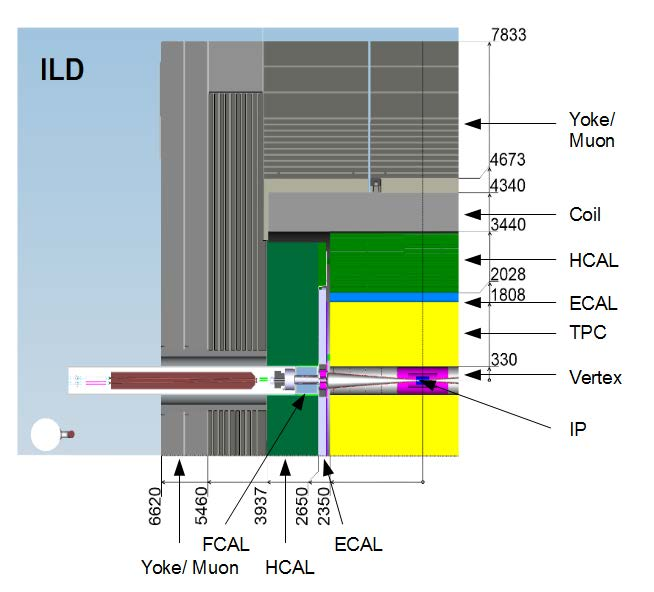
\includegraphics[width=\textwidth]{ILD/ILD}
    \caption{}
    \label{fig:ILD}
  \end{subfigure}
  \begin{subfigure}[b]{0.35\textwidth}
    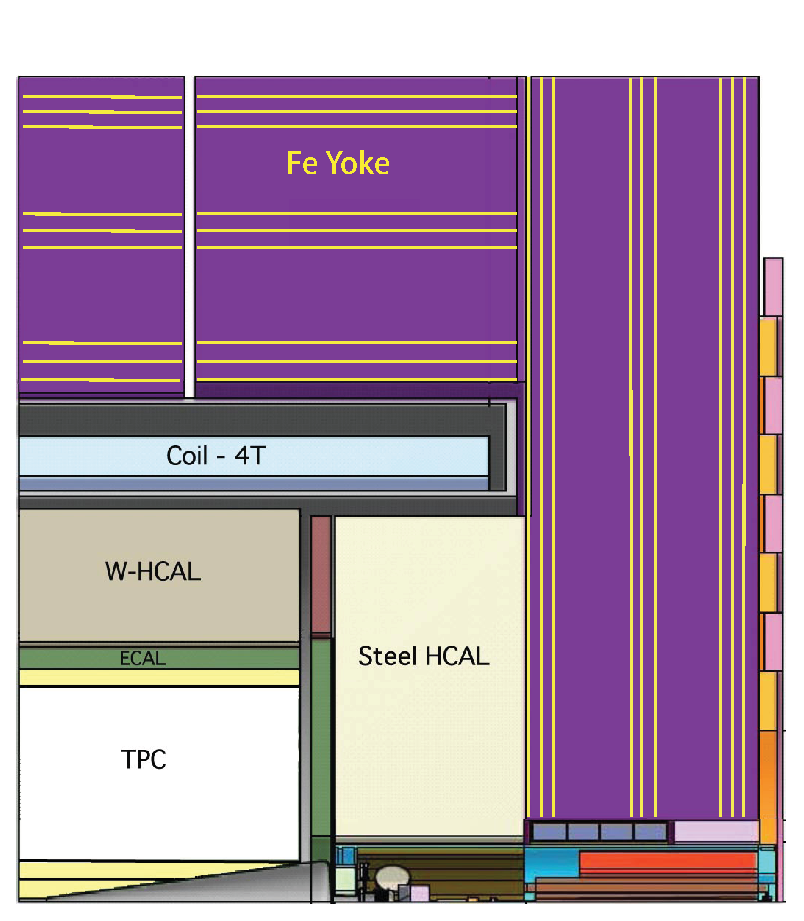
\includegraphics[width=\textwidth]{ILD/CLIC_ILD}
    \caption{}
    \label{fig:CLIC_ILD}
  \end{subfigure}
\caption[]
{\FIGURE{fig:ILD} and \FIGURE{fig:ILD} shows longitudinal cross section of top quadrant of the \ILD and the \CLICILD detector concepts, taken from \cite{Baer:2013cma} and \cite{Linssen:2012hp} respectively. From interaction point (\IP) outwards, there is a tracking system compromising a large time projection chamber (\TPC) augmented with silicon tungsten layer, highly granular electromagnetic calorimeters (\ECAL) and hadronic calorimeters (\HCAL), muon chambers, forward calorimeters (\FCAL), magnetic coils and iron yokes. Numbers are in units of mm.}
\label{fig:detectorILD}
\end{figure}




\section{Overview of \ILD sub-detectors}

The \ILD detector concept is designed as a general purpose detector. Closest to the interaction points are the precision a vertex detector and a tracking system. The tracking system consists of silicon tracking with a time projection chamber. Surrounding the tracking system is a high granular calorimeter system. The outer solenoid provides a magnetic field of 3.5\,T. The most outer iron return yoke acts as a muon calorimeter.


\section{Vertex Detector}

The pixel-vertex detector(\VTX) needs to be close to the interaction point to reconstruct secondary vertex. As the \TPC is the main tracking  detector, the \VTX mainly measures the impact parameter of tracks. The structure is three double layers with a barrel geometry. Double layer lowers the material budget and improves the impact parameter measurements. The first double layer is half length of the other two to avoid the high occupancy region of direct low omentulum hits from the incoherent pair background.

For the \CLIC, the same structure is used. The first layer is moved outwards due to a larger high occupancy region with higher centre-of-mass energy. The detector is also required to provided time stamping at nanoseconds level.


\section{Tracking Detectors}

The hybrid  tracking system is consists of a large volume time projection chamber (\TPC), a Silicon Inner Tracker (\SIT), a Silicon External Tracker (\SET) in the barrel region, a end cap tracking component (\ETD) behind the endplate of the \TPC, and a silicon forward tracker (\FTD) in the forward region. The \SIT, \SET, and \ETD are made up two single-sided strip layers tilted by a small angle. The \FTD is a system of two silicon-pixel disks and five silicon-strip disks.  The silicon envelope tracking system and the \TPC are shown in \Figure{fig:detectorTracking}.


The main part of the tracking system, the \TPC, can measure a large number of three dimensional spatial points. Continuous tracking allows precise reconstruction of non-pointing tracks. The \TPC is optimised for point resolution and minimum material, as required for the best calorimeter and particle flow performance.

The barrel silicon trackers improve the the overall momentum resolution. They provide additional high precision space points and additional redundancy between the \TPC, the \VTX, and the calorimeters. The \FTD provide the low angle coverage which is not covered by the \TPC.

For the \CLICILD, the hybrid structure is used. The outer silicon tracking system is more important at the \CLIC to achieve a high momentum resolution at high centre-of-mass energy, as it is challenging using a \TPC to sperate two tracks in high energy jets and to identify events in the collection of 312 bunch crossings in 156\,ns.



\begin{comment}
A system of silicon strip and pixel detectors surrounds the VTX detector. In the barrel, two
layers of silicon strip detectors (SIT) are arranged to bridge the gap between the VTX and the TPC.
In the forward region, a system of two silicon-pixel disks and five silicon-strip disks (FTD) provides
low angle tracking coverage.

The barrel silicon parts SIT and SET provide precise space points before and after the TPC; this
improves the overall momentum resolution, helps in linking the VTX detector with the TPC, and
in extrapolating from the TPC to the calorimeter. The coverage of the TPC with silicon tracking
is completed by the ETD, located within the gap separating the TPC and the end-cap calorimeter.
Together these systems help in calibrating the overall tracking system, in particular the TPC. The
good timing resolution of the silicon detectors relative to the time between bunches in the ILC together
with the high spatial precision helps in time-stamping tracks and assigning them to a given bunch
within an ILC bunch train.
\end{comment}


\begin{figure}[tdbph]
\centering
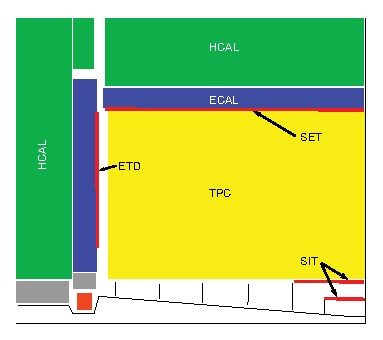
\includegraphics[width=0.45\textwidth]{ILD/Tracking}
\caption[]
{A top quadrant view of the \ILD silicon envelope system, \SIT, \SET, \FTD, and \ETD as included in MOKKA full simulation, adapted from the figure in \cite{Baer:2013cma}.}
\label{fig:detectorTracking}
\end{figure}


\section{Electromagnetic Calorimeter}

The Silicon-Tungsten sampling electromagnetic calorimeters in the \ILD consist of a nearly cylindrical barrel and two end cap systems, optimised for particle flow. The \ECAL measures photon energies and separates photons from other particles. The fine granular \ECAL also sits inside the \HCAL, which hosts the first part of the hadronic showers and greatly helps to separate hadronic showers. 

The particle flow paradigm has a large impact on the \ECAL design with many requirements. In addition for the \ECAL to measure and separate photons, it also needs to reconstruct detail shower profiles to separate electromagnetic showers from hadronic showers, as approximately 50\% of hadronic showers starts in the \ECAL. These requirements can be fulfilled with an excellent three dimensional granular \ECAL.

From test beam data and simulation studies, a sampling calorimeter with longitudinal and transverse segmentation below one Moli\`{e}re radius and below one radiation length at the front the calorimeter is needed. The most compact design is realised with Tungsten as absorber material and silicon pad diodes as active material. A cross section of the \ECAL is shown in \Figure{fig:detectorILDECAL}. Tungsten is a dense material with a large ratio of interaction length to radiation length. This helps to separate electromagnetic showers from hadronic showers by delaying the start of the hadronic showers. Silicon pad size of 5.1 by 5.1 \,mm cover large areas. They are simple and reliable to operate. The choice of thin silicon layers offers a great spatial resolution at a cost of the energy resolution in favour of the particle flow.

The longitudinal segregation is a compromise between the cost and the performance. The total 30 layers, which is about 20\,cm, provides about 24 radiation lengths. The first 20 layers use 2.1\,mm thick absorber plates, which is twice finer sampling than the last 10 layers with 4.2\mm thick absorber plates. The test beam data with electron shows the energy resolution of the \ECAL concept to be $16.6/\sqrt{E(\ GeV)}\oplus1.1\%$, which is compatible with the values assumed for the full \ILD detector simulation.

For the \CLICILD, the same \ECAL from the \ILD is assumed, as the requirements of a \CLIC detector are satisfied. The increased centre-of-mass energy results in extra energy leakage. But only a small fraction of particles are affected and the leakage is controlled by the \HCAL.

\begin{figure}[tdbph]
\centering
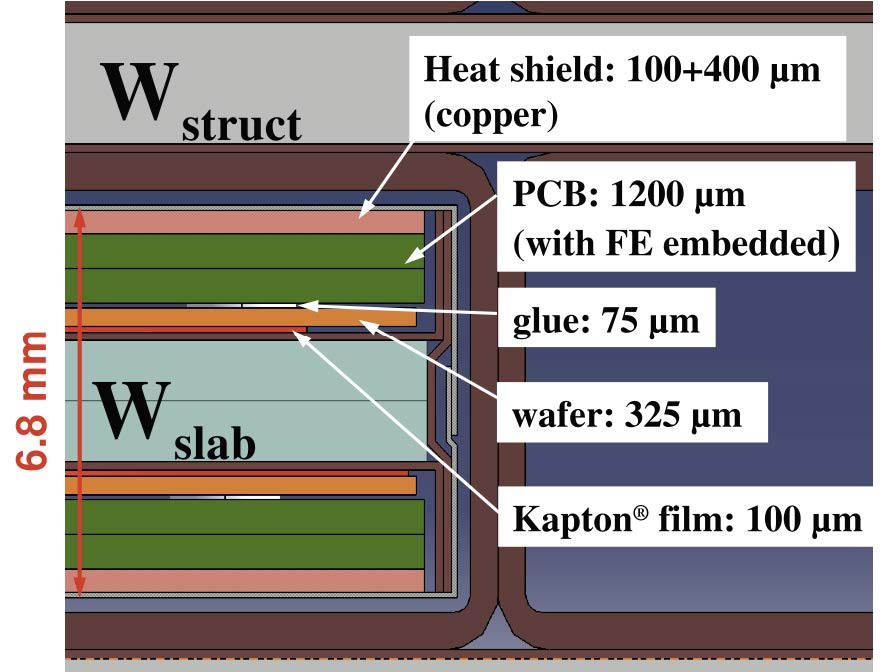
\includegraphics[width=0.45\textwidth]{ILD/ILD_ECAL}
\caption[]
{A cross section through electromagnetic calorimeter layers, taken from \cite{Baer:2013cma}.}
\label{fig:detectorILDECAL}
\end{figure}

\begin{comment}
The particle flow paradigm has a large impact on the design of the electromagnetic calorimeter system.
A key requirement is the capability of the system to separate overlapping showers from each other.
A calorimeter for particle flow thus needs to be able to do pattern recognition in the shower. The
electromagnetic section has a number of tasks to fulfill. It should be able to reconstruct photons
in the presence of close-by particles. It should be able to reconstruct the detailed properties of the
shower, such as shower shape, starting point and energy to distinguish early starting electromagnetic
showers from hadronic ones. It should be noted that about half of the hadronic showers start inside
the electromagnetic calorimeter. Thus an excellent three-dimensional granularity of the device is of
utmost importance.

The transverse and longitudinal segmentation of both calorimeters has been optimised based on
detailed simulation and test beam data. It has been shown that the granularity must be of the order
of X0 in all three dimensions. This implies that a sampling calorimeter is the best option for both
ECAL and HCAL. For the ECAL the most compact design can be realised with tungsten as absorber
material. For the HCAL iron is chosen as this allows an excellent energy resolution for hadrons at
manageable granularity.
For the ECAL, silicon pad diodes lead to the highest possible compactness (and effective Moli`ere
radius) and exhibit excellent stability of calibration. As an option scintillating strips with silicon
photo-sensor readout are studied, which provide a similar effective segmentation. The two technologies
can be combined in order to reach a cost-performance optimum.

In order to have a better separation of close-by showers in the calorimeter, a system with a
small Moli`ere radius is advantageous. Further help in the separation between electromagnetic and
hadronic showers can come from a large ratio between interaction length and radiation length. A
small radiation length will move the start of the electromagnetic shower earlier in the calorimeter,
while a large interaction length will reduce the fraction of hadronic showers starting in the ECAL.

The particle flow approach requires that the calorimeters are placed inside the magnetic coil,
see Sec. 1.2. This has a major impact on the layout of the detector, and on the cost. Therefore, a
compact calorimeter is preferred in order to minimise the overall physical thickness, which in turn
reduces the size of the coil. For the ECAL tungsten is a good choice for the radiator as it is dense, and
has a large ratio of interaction length to radiation length. The final system layout is a compromise
between performance and cost. The energy resolution scales with OT, where T is the individual
absorber plate thickness, while the cost scales linearly with the surface area of the readout layers. For
ILD a solution with 30 readout layers and a thickness of the ECAL of 24X0 has been chosen as the
baseline. The optimisation of the layout is ongoing.

For a chosen pad size of 5 . 5mm2 silicon pin diodes are a good choice. They can cover large
areas, are reliable and simple to operate, allow for a thin readout layer and can operate in the 3.5 T
strong central magnetic field. While the very thin silicon layers offer excellent performance for the
tracking capabilities of the calorimeter, the energy resolution is somewhat degraded. Here a less
compact device, with a thicker readout layer, will show better performance.

The requirements on granularity, compactness and particle separation lead to the choice of a
sampling calorimeter with tungsten (radiation length X0 = 3.5 mm, Moliere Radius RM = 9 mm and
interaction length = 99 mm) as absorber material. This allows for a compact design with a depth
of roughly 24 X0 within 20 cm and, compared to e.g. lead, a better separation of electromagnetic
showers generated by near-by particles. To achieve an adequate energy resolution, the ECAL is
longitudinally segmented into 30 layers, possibly with varying tungsten thicknesses. In order to
optimise the pattern recognition performance, the active layers (either silicon diodes or scintillator)
are segmented into cells with a lateral size of 5 mm.
\end{comment}

\section{Hadronic Calorimeter}

The requirements of sampling hadronic calorimeter is, again, driven by the need of the particle flow. The need of three dimensional granularity in transverse and logistically direction is satisfied by a sampling calorimeter. 

  

The principle role of the \HCAL is to separate neutral hadron showers from other particles, and to measure neutral hadron energies. The neutral hadron contribution of  the jet energy is around 10\% on average. A moderate fine  granular \HCAL is a good balance between cost and performance. The chosen layout is 48 longitudinal layers with 3 by 3\cm scintillator tiles, using an analogue read out system. The layout is shown in \Figure{}.

The longitudinal system provide about 6 radiation lengths including the \ECAL, which is sufficient to contain the hadronic showers. The transverse cell sizes has been optimised for the best jet energy resolution. It is found that no substantial gain below 3\,cm and performance degradation above 3\,cm. Hence 3\,cm cell size is chosen for the \HCAL. The jet energy resolution as a function of \HCAL scintillator cell size with different jet energies is shown in \Figure{}.

The absorber material, stainless steel is chosen for mechanical and calorimetric reasons. Steel allows a self-supporting structure without auxiliary supports. Also steel has a moderate ratio of interaction length to radiation length.

For the \CLICILD, extra layers are added to contain the hadronic shower at high energy. The increased thickeners is justified by the simulation studies, where the jet energy resolution degrades quickly for a thinner \HCAL.

\begin{comment}
The role of the HCAL is to separate the deposits of charged and neutral hadrons and to precisely
measure the energy of the neutrals. Their contribution to the jet energy, around 10% on average,
fluctuates over a wide range from event to event, and the accuracy of the measurement is the
dominant contribution to the particle flow resolution for jet energies up to about 100 GeV. For higher
energies, the performance is dominated by confusion, and both topological pattern recognition and
energy information are important for correct track cluster assignment.


This is followed by a highly segmented hadronic calorimeter (HCAL) with up to 48 longitudinal
samples and small transverse cell size. Two options are considered, both based on a Steel-absorber
structure. One option uses scintillator tiles of 3 . 3 cm2, which are read out with an analogue
system. The second uses a gas-based readout which allows a 1.1 cm2 cell geometry with a binary or semi-digital readout of each cell.


The HCAL is optimized to measure neutral hadrons
well and thus has to provide the topological resolution power for separating them from the showers of
the much more abundant charged hadrons which must be matched with tracks.


The transverse and longitudinal segmentation of both calorimeters has been optimised based on
detailed simulation and test beam data. It has been shown that the granularity must be of the order
of X0 in all three dimensions. This implies that a sampling calorimeter is the best option for both
ECAL and HCAL. For the ECAL the most compact design can be realised with tungsten as absorber
material. For the HCAL iron is chosen as this allows an excellent energy resolution for hadrons at
manageable granularity.



The role of the HCAL is to separate the deposits of charged and neutral hadrons and to precisely
measure the energy of the neutrals. Their contribution to the jet energy, around 10% on average,
fluctuates over a wide range from event to event, and the accuracy of the measurement is the
dominant contribution to the particle flow resolution for jet energies up to about 100 GeV. For higher
energies, the performance is dominated by confusion, and both topological pattern recognition and
energy information are important for correct track cluster assignment.




The HCAL is conceived as a sampling calorimeter with steel absorber and scintillator tiles
(analogue HCAL) or gaseous devices (semi-digital HCAL) as active medium. Due to the rigidity of
stainless steel, a self-supporting structure without auxiliary supports (dead regions) can be realised.
Moreover, in contrast to heavier materials, iron with its moderate ratio of hadronic interaction length
(.I = 17 cm) to electromagnetic radiation length (X0 = 1.8 cm) allows a fine longitudinal sampling
in terms of X0 with a reasonable number of layers in a given total hadronic absorption length, thus
keeping the detector volume and readout channel count at an acceptable level. This fine sampling is
beneficial both for the measurement of the sizeable electromagnetic energy part in hadronic showers
and for the topological resolution of shower substructure, needed for particle separation and weighting.
Two baseline technology options have been developed, the scintillator-tile based AHCAL and the
Glass Resistive Plate Chamber (GRPC) based SDHCAL.
\end{comment}



This section will describe sub-systems from small to large radius.



\begin{comment}
The International Large Detector (ILD) is a concept for a detector at the International Linear Collider,
ILC [198]. In a slightly modified version, it has also been proposed for the CLIC linear collider [199].
The ILD detector concept has been optimised with a clear view on precision. In recent years
the concept of particle flow has been shown to deliver the best possible overall event reconstruction.
Particle flow implies that all particles in an event, charged and neutral, are individually reconstructed.
This requirement has a large impact on the design of the detector, and has played a central role in
the optimisation of the system. Superb tracking capabilities and outstanding detection of secondary
vertices are other important aspects. Care has been taken to design a hermetic detector, both in
terms of solid-angle coverage, but also in terms of avoiding cracks and non-uniformities in response.
The overall detector system has undergone a vigorous optimisation procedure based on extensive
simulation studies both of the performance of the subsystems, and on studies of the physics reach
of the detector. Simulations are accompanied by an extensive testing program of components and
prototypes in laboratory and test-beam experiments.
Figure III-1.1
View of the ILD detector
concept.
The ILD detector concept has been described in a number of documents in the past. Most
recently the letter of intent [198] gave a fairly in depth description of the ILD concept. The ILD
concept is based on the earlier GLD and LDC detector concepts [200, 201, 202]. Since the publication
of the letter of intent, major progress has been made in the maturity of the technologies proposed for
ILD, and their integration into a coherent detector concept
\end{comment}

\section{Motivation}



Photon - passage through matter. Photon electromagnetic shower


Since Higgs discovery in the \LHC in 2012, Higgs



Ha there is a higgs.

We found higgs. Higgs is cool. It explains mass.

Why double higgs. Double higgs coulpling is unique to linear collider. It can revel much about the BSM models.

Generator level study has performed. ILC has done this this and that. gHHH in CLIC before

Here we do things differently. First subchannels, then extract both couplings simultaneously.

